\documentclass[aspectratio=43,unicode,10pt]{beamer}
\usetheme{ttipresentation}

\usepackage{graphicx}
\usepackage{multicol}

\beamertemplatenavigationsymbolsempty

\newcommand{\itemtitle}[1]{\textbf{#1}\\}
\newcommand{\fire}[1]{\textcolor{red}{\textbf{#1}}}
\newcommand{\freeze}[1]{\textcolor{blue}{\textbf{#1}}}
\newcommand{\then}{\textcolor{ttiblue}{\textbf{⇒}}\hspace{1ex}}
\newcommand{\good}{\textcolor{orange}{\textbf{◎}}\hspace{1ex}}
\newcommand{\arrow}{\textcolor{ttiblue}{\textbf{→}}\hspace{1ex}}
\newcommand{\set}[1]{\{#1\}}


\title[font2char2word2sent2doc]{
  The New Model for Sentiment Classification \\
  of Documents Exploiting Fonts}
\institute[CoIn Lab., TTI]{Computational Intelligence Laboratory, \\
                      Toyota Technological Institute}
\author{16423 Yota Toyama}
\date{\today}



\begin{document}

\begin{frame}
\titlepage
\end{frame}

\begin{frame}{Sentiment classification of documents}
  \begin{itemize}
    \item A task to classify document into some sentiment classes
    \item Do this with machine learning!
    \item Purpose: find the best function,
          f: \set{document}\rightarrow\set{sentiment label}
    \item Example: predicting a number of stars given by a user
                   from the review text
  \end{itemize}
  \begin{figure}
    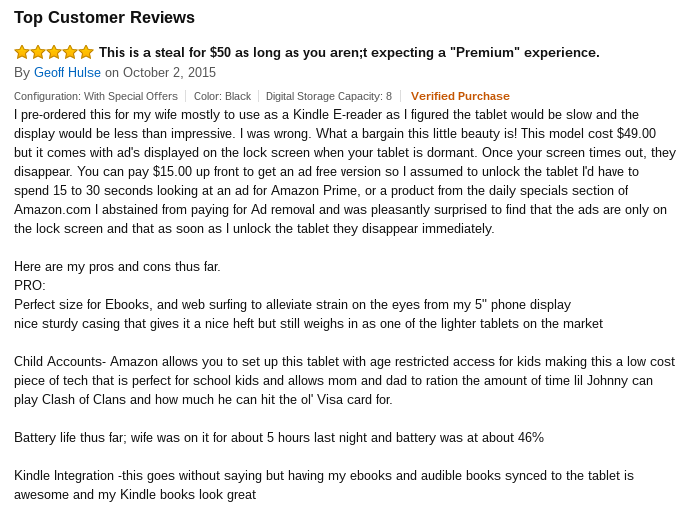
\includegraphics[width=0.6\linewidth]{fig/review.png}
  \end{figure}
\end{frame}

\begin{frame}{The proposed method}
  \begin{figure}
    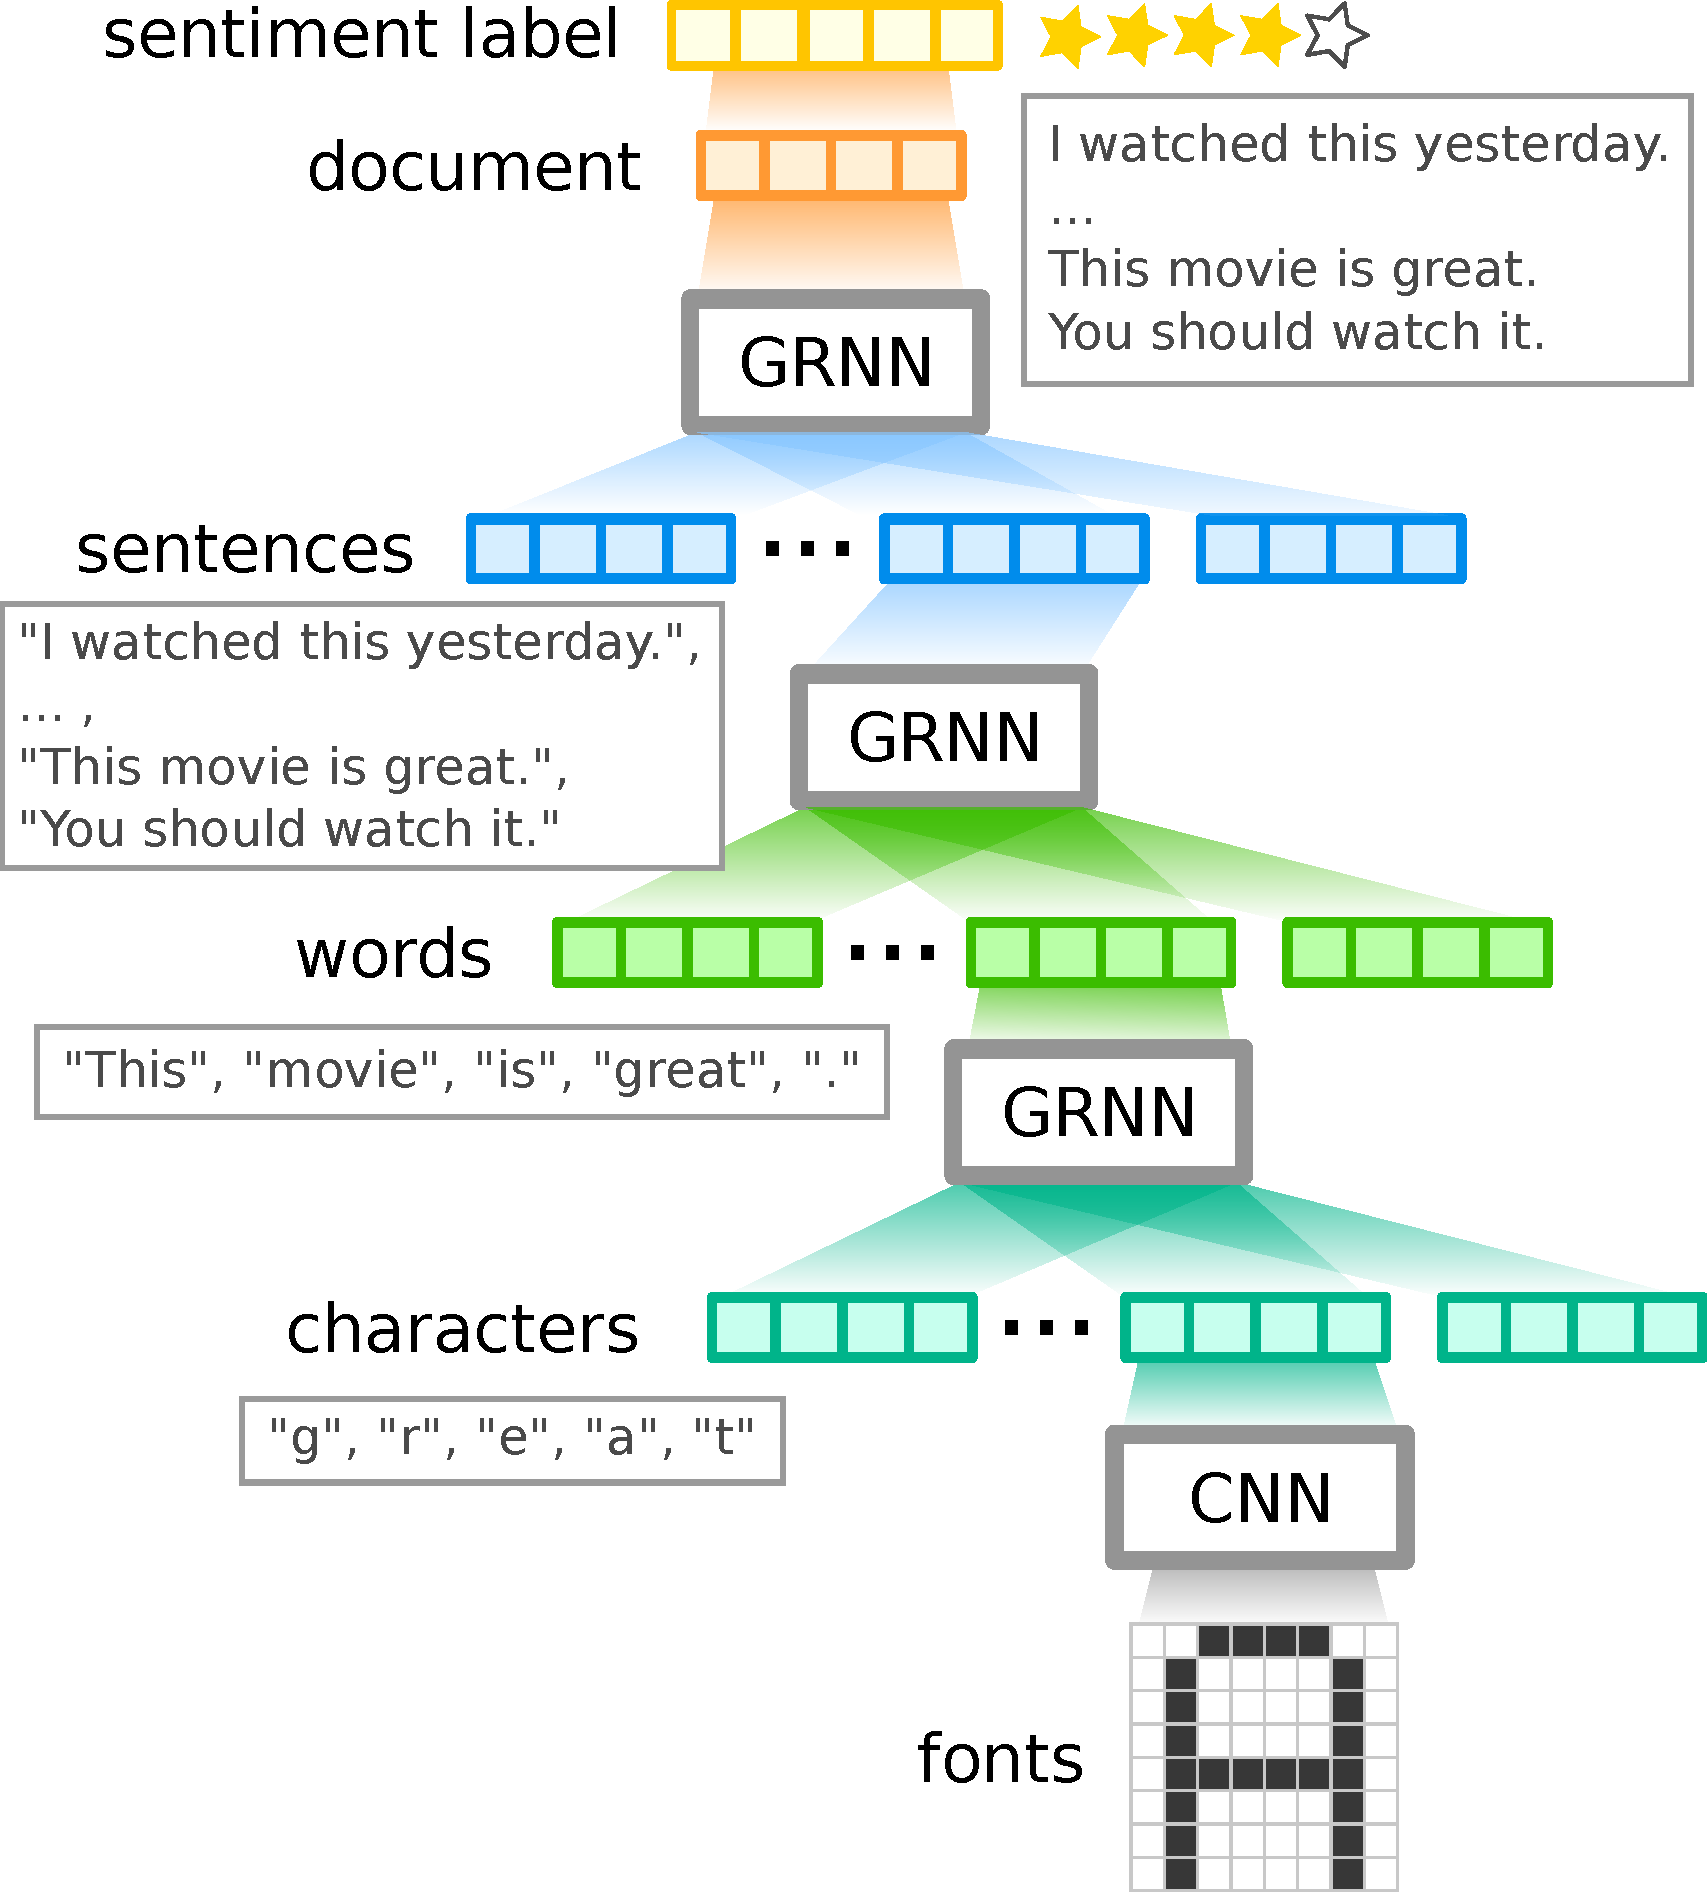
\includegraphics[width=0.6\linewidth]{fig/fcwsd.pdf}
  \end{figure}
\end{frame}

\begin{frame}{Results}
  \begin{itemize}
    \item Our model is not working well yet ...
    \item The below is the result of the model equal
          to our model without fonts.
    \item The state-of-the-art accuracy: \sim 94\%
    \item More effort will be needed.
  \end{itemize}
  \begin{figure}
    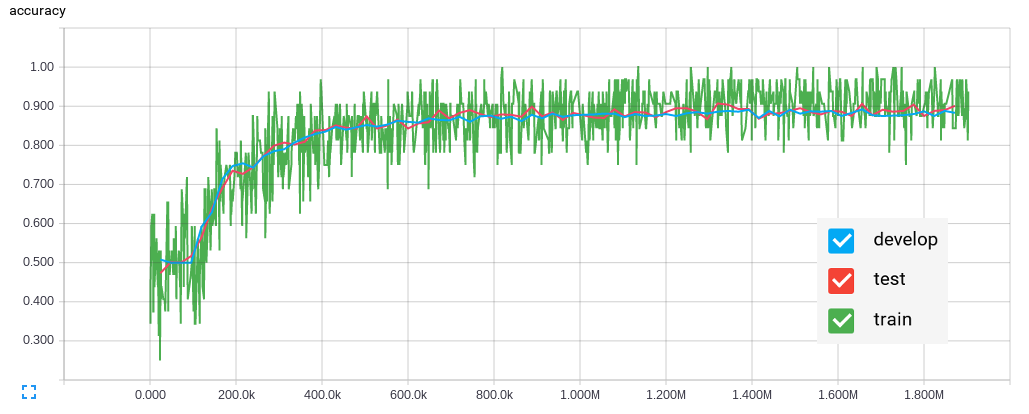
\includegraphics[width=\linewidth]{fig/cwsd_learning.png}
  \end{figure}
\end{frame}

\end{document}
